\documentclass[a4paper]{extarticle}
\usepackage[utf8]{inputenc}
\usepackage[a4paper, margin=1in]{geometry}

\usepackage{amssymb}
\usepackage{amsmath}
\usepackage{enumitem}
\usepackage{tcolorbox}
\usepackage{fancyhdr}
\usepackage{graphicx}
\usepackage{float}

\setlength{\parindent}{0em}
\setlength{\parskip}{0.4em}

\definecolor{theoremblue}{RGB}{1, 73, 124}
\definecolor{corollaryblue}{RGB}{70, 143, 175}
\definecolor{exampleblue}{RGB}{137, 194, 217}

\newtcolorbox{tbox}{colback=theoremblue!20,colframe=theoremblue,
boxrule=0pt,arc=0pt,boxsep=2pt,left=2pt,right=2pt,leftrule=2pt}

\newtcolorbox{cbox}{colback=corollaryblue!20,colframe=corollaryblue,
boxrule=0pt,arc=0pt,boxsep=2pt,left=2pt,right=2pt,leftrule=2pt}

\newtcolorbox{ebox}{colback=exampleblue!20,colframe=exampleblue,
boxrule=0pt,arc=0pt,boxsep=2pt,left=2pt,right=2pt,leftrule=2pt}

\title{EnpRisk - Lecture Notes Week 2}
\author{Ruben Schenk, ruben.schenk@inf.ethz.ch}
\date{\today}

\pagestyle{fancy}
\fancyhf{}
\rhead{ruben.schenk@inf.ethz.ch}
\rfoot{Page \thepage}
\lhead{EnpRisk - Lecture Notes Week 2}

\begin{document}

\maketitle
\newpage

\subsubsection{Definition of Risk}

It is important to make the following distinctions:

\begin{itemize}
    \item Distinction between risk and uncertainty: Risk = Uncertainty + Damage
    \item Distinction between risk and hazard: Risk = Hazard / Safeguard
\end{itemize}

\textbf{Risk assessment} consists of hazard identification, event probability assessment, and consequence assessment. \textbf{Risk control} requires the definition of acceptable and comparative evaluation through monitoring and decision analysis. Risk control also includes failure prevention and consequence mitigation. \textbf{Risk communication} involves perceptions of risk and depends on the audience targeted.

One last important point to consider are \textbf{human errors.} Human errors are unwanted circumstances caused by humans that result in deviations from the expected norms that place systems at risk. Human error identification techniques should provide a comprehensive structure for determining significant human errors within the system:

\begin{itemize}
    \item \textbf{Human error modelling:} Currently, there is no consensus on how to model humans reliably. The human error estimates are often based on simulation tests, models, and expert estimation.
    \item \textbf{Human error quantification:} Still a developing science requiring understanding of human performance, cognitive processing, and human perceptions.
\end{itemize}

\subsection{The Big Problems}

Econometric analysis of growth in the USA, Japan, and Germany between 1960 and 1996 shows that \textit{energy drives about 50\% of economic growth.} Mainstream economics, on the other hand, gives energy only a weight of 5\% according to energy's share in the total cost of the production factors capital, labor, and energy.

Energy is just one of many factors, such as water, erosion, melting ice, overpopulation, etc. Those other factors, however, were left out during the lecture. They will be added to the summary if deemed necessary for the exam.

\section{Start-Ups and Investment in Innovation}

\subsection{Landscape on Entrepreneurship and Private Investment}

We start by looking at the difference between \textbf{private equity} and \textbf{venture capital.}

\subsubsection{Private Equity}

\begin{itemize}
    \item Financing mainly used to buy mature well-established companies
    \item Always a combination of debt and equity (shares)
    \item Value created through streamlining of operations, cost-cutting, consolidation, etc.
    \item Strong focus on cash flow to pay off debt, companies are highly leveraged
    \item Leverage increases risk profile but also potential return
\end{itemize}

\[
    Asset = Debt + Equity \qquad Leverage = \frac{Asset}{Equity}
\]

\subsubsection{Venture Capital}

\begin{itemize}
    \item Financing mainly given to startup companies and small businesses
    \item Value created through growth
    \item Growth expected from innovation, disruptive technology, new products, etc.
    \item Very high risk profile, no cash flow but cash burn
    \item Company can only finance through equity, often the risk profile is too high to get debt financing
\end{itemize}

Most businesses do not survive the first five years (roughly 50\%). Roughly 80\% survive past the first year. Investors want to manage their risk with \textbf{preference shares} and by gaining as much \textbf{control} as possible on the company, through shareholder agreements, voting rights, board membership, etc.

In the event of the failure of the company, preferred shareholders may receive payment from liquidation before common shareholders. When the company is sold, preferred shareholders may receive payment in full before the common shareholders (sometimes with a guaranteed \textbf{return on investment (ROI)}).

Investors must be \textbf{detached} from individual companies and look at the whole portfolio. \textit{This is not aligned with the Entrepreneur's viewpoint.}

There is a complex relationship between risk and return. The simple representation is: higher risk leads to larger return.

However, the nature of risk is tricky. Take as an example the UK stock market bubble ending in October 1987. The volatility is low at the crest of the bubble and high at the end of the crash. When is the desired entry point? At low or at high volatility?

In summary, both entrepreneurs and investors want to be in control, but they have very different viewpoints:

\begin{figure}[H]
    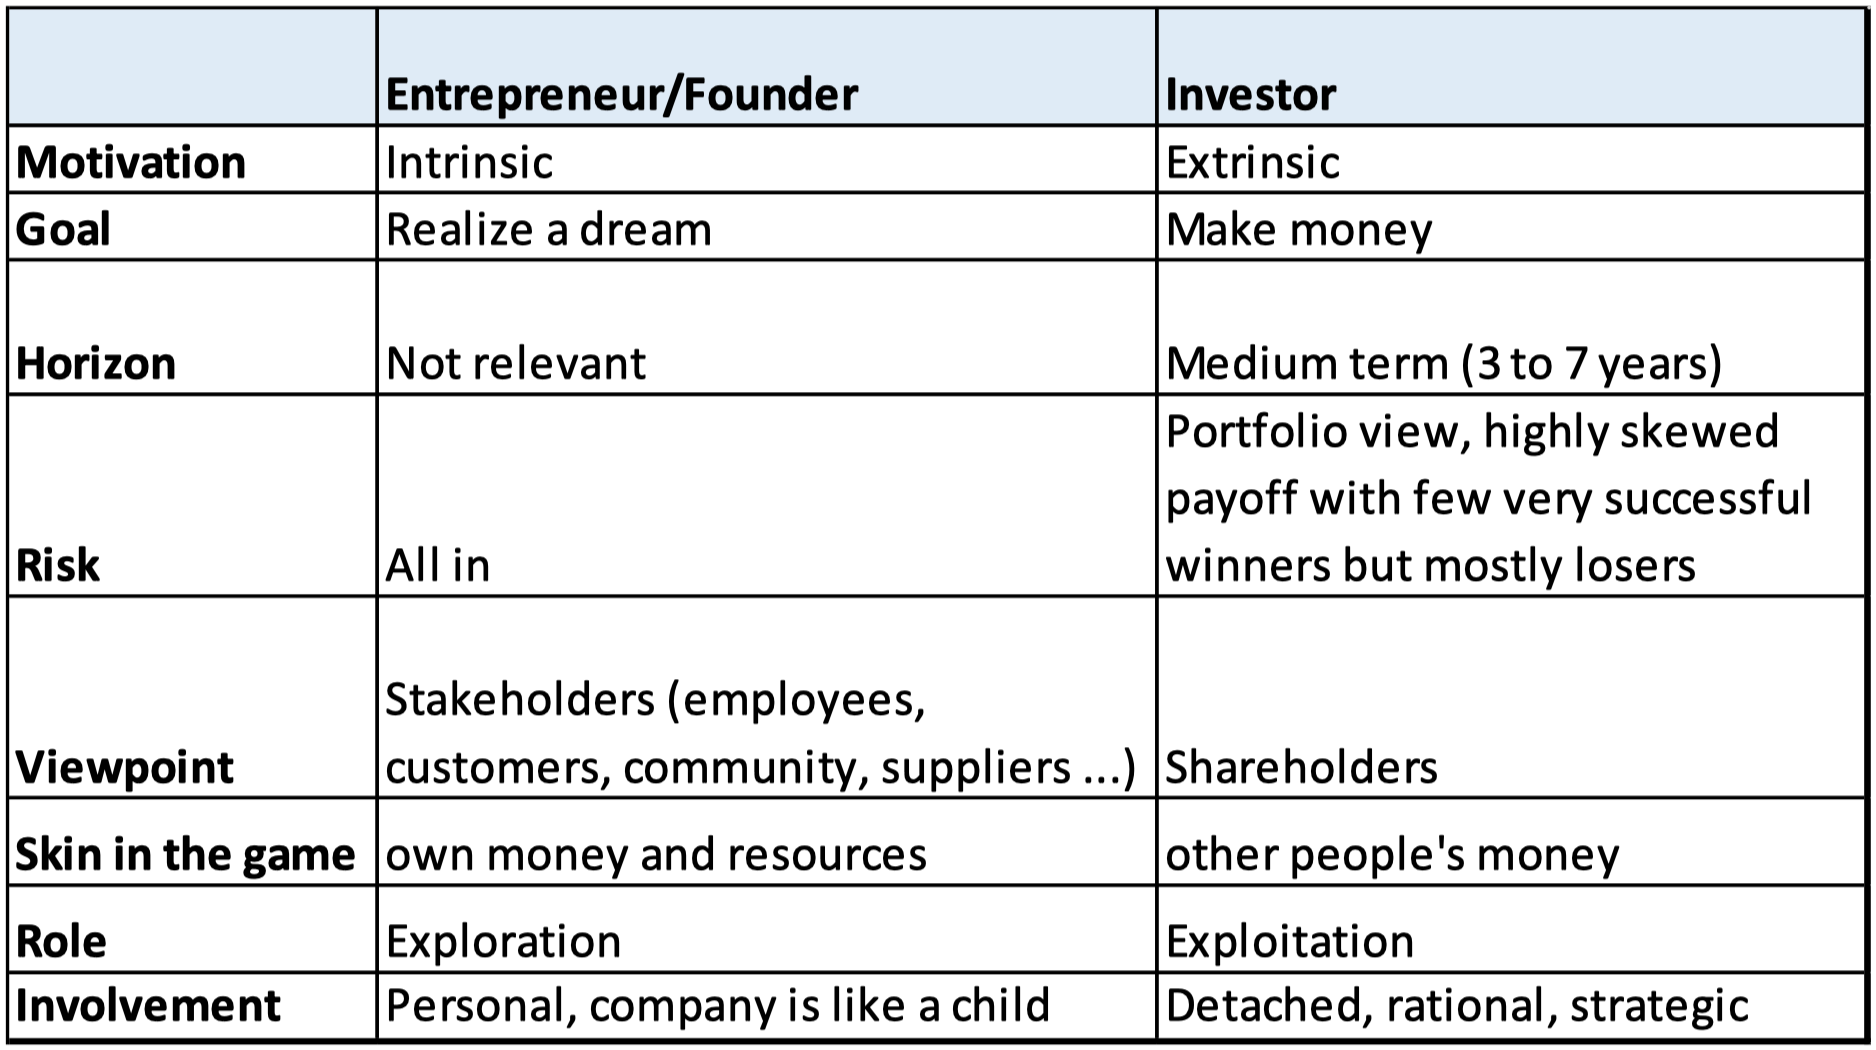
\includegraphics[width=13cm]{../images/EnpRisk_Fig2-1}
    \centering
\end{figure}

The challenges of exploration can be summarized by some exploration requirements according to Herbert Simon:

\begin{itemize}
    \item Tolerance of ambiguity/uncharted territory
    \item Patience: Learning-by-doing, accumulation of knowledge, and trial-and-error
    \item Luck/serendipity
    \item Persistence/diligence
    \item Intuition: Use of smart heuristics
\end{itemize}

It is important to realize that exploitation is tempting from a short-term risk/return perspective, but there are serious caveats on the long run. Disruptive innovations are initially too small to meet the ROI-targets of large established firms. However, they steadily work their way up eventually capitalizing on a crucial first-mover advantage against large, less nimble, market leaders.

Some serious \textbf{pitfalls} to consider:

\begin{itemize}
    \item Overconfidence
    \item Framing
    \item Base-rate neglect
    \item Availability cascades
    \item Substitution
    \item Halo
    \item Sunk cost effect
    \item Stereotyping
    \item etc.
\end{itemize}

\end{document}